\documentclass{beamer}
\mode<presentation>
\usepackage{amsmath}
\usepackage{amssymb}
%\usepackage{advdate}
\usepackage{graphicx}
\graphicspath{{../Figs/}}
\usepackage{adjustbox}
\usepackage{subcaption}
\usepackage{enumitem}
\usepackage{multicol}
\usepackage{mathtools}
\usepackage{listings}
\usepackage{url}
\def\UrlBreaks{\do\/\do-}
\usetheme{Boadilla}
\usecolortheme{lily}
\setbeamertemplate{footline}
{
  \leavevmode%
  \hbox{%
  \begin{beamercolorbox}[wd=\paperwidth,ht=2.25ex,dp=1ex,right]{author in head/foot}%
    \insertframenumber{} / \inserttotalframenumber\hspace*{2ex} 
  \end{beamercolorbox}}%
  \vskip0pt%
}
\setbeamertemplate{navigation symbols}{}
\let\solution\relax
\usepackage{gvv}
\lstset{
%language=C,
frame=single, 
breaklines=true,
columns=fullflexible
}

\numberwithin{equation}{section}
\begin{document}


\title{5.11.1}
\author{AI25BTECH11002 - Ayush Sunil Labhade}
{\let\newpage\relax\maketitle}


\textbf{Question}: Determine the loop currents in Fig. 5.11.1.1.
\begin{figure}[H]
    \centering
    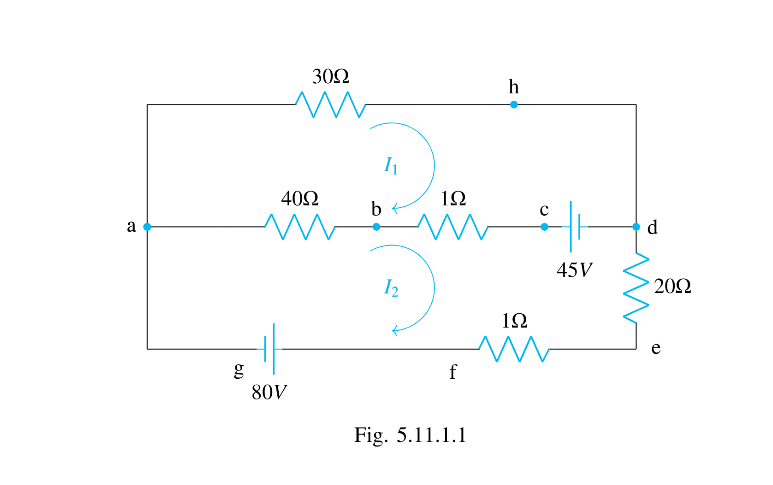
\includegraphics[width=\columnwidth]{5.11.1.1.png}
    \label{Circuit}
\end{figure}

\newpage
\textbf{Solution:}\\

Using mesh current analysis with Kirchhoff's Voltage Law (KVL):\\

Let the loop currents be $I_1$ and $I_2$ as shown in Fig.~5.11.1.1.\\

\textbf{Applying KVL to loop (a-b-c-d-h-a):}
\begin{align}
30I_1 + 40(I_1 - I_2) + 1(I_1 - I_2) - 45 = 0
\end{align}
\begin{align}
\Rightarrow 71I_1 - 41I_2 = 45
\end{align}

\textbf{Applying KVL to loop (a-b-c-d-e-f-g-a):}
\begin{align}
40(I_2 - I_1) + 1(I_2 - I_1) + 20I_2 + 1I_2 - 80 + 45 = 0
\end{align}
\begin{align}
\Rightarrow -41I_1 + 62I_2 = 35
\end{align}

Hence, the two mesh equations are:
\begin{align}
	71I_1 - 41I_2 &= 45
\end{align}
\begin{align}
	-41I_1 + 62I_2 &= 35
\end{align}

Let 
\[
\vec{M} = \myvec{71 & -41 \\ -41 & 62}, \quad 
\vec{x} = \myvec{I_1 \\ I_2}, \quad 
\vec{V} = \myvec{45 \\ 35}
\]
$\therefore$ for finding $I_1$ and $I_2$
\begin{align}
\vec{M}\vec{x} = \vec{V}
\end{align}

\begin{align}
\myvec{71 & -41 \\ -41 & 62}\myvec{I_1 \\ I_2} = \myvec{45 \\ 35}
\end{align}

\textbf{Solving by Row Transformations:}
\begin{align}
	\augvec{2}{1}{
71 & -41 & 45 \\
-41 & 62 & 35
}
\end{align}
Row Transformation-1: $R_2 \rightarrow 71R_2 + 41R_1$
\begin{align}
	\augvec{2}{1}{
71 & -41 & 45 \\
0 & 2831 & 3820
	}
I_2 = \frac{3820}{2831} = 1.35\,A
\end{align}

Substitute in (1):
\begin{align}
71I_1 - 41(1.35) = 45\\
\Rightarrow I_1 = 1.52\,A
\end{align}

\sbrak{
I_1 = 1.52\,A,\quad I_2 = 1.35\,A
}
\end{document}
